%-------------------------------------------------------------------------------
% File:		    Report.tex
% Author:	    Igor Janjic, Danny Duangphachanh, Leah Krynitsky, Brian
%               Hilnbrand
% Description:	[ECE 4534] Embedded Systems Design
%		        Project proposal.
%%------------------------------------------------------------------------------ 

\input{./Preamble.tex}
\input{./Definitions.tex}
\input{./Programming.tex}

% Make compact sections.
\usepackage[compact]{titlesec}

\begin{document}

%-------------------------------------------------------------------------------
% File:		    Title.tex
% Author:	    Igor Janjic
% Description:	[ECE 4564] Network Applications Design
%		        Project proposal.
%%------------------------------------------------------------------------------

\begin{titlepage}

\centering
\vspace*{\baselineskip}

\rule{\textwidth}{1.6pt}\vspace*{-\baselineskip}\vspace*{2pt}
\rule{\textwidth}{0.4pt}\\[\baselineskip]

{\LARGE Final Report\\[0.3\baselineskip]}

\rule{\textwidth}{0.4pt}\vspace*{-\baselineskip}\vspace{3.2pt}
\rule{\textwidth}{1.6pt}\\[\baselineskip]

\wl

\scshape Due December 12, 2014 at 11:55 PM.
{\small 
\\[\baselineskip]\par}

\vfill

Created by:\\[0.2\baselineskip]
{Brian Hilnbrand:     \texttt{brhiln@vt.edu}}\\[0.2\baselineskip]
{Danny Duangphachanh: \texttt{bboydd@vt.edu}}\\[0.2\baselineskip]
{Igor Janjic:         \texttt{ijanjic@vt.edu}}\\[0.2\baselineskip]
{Leah Krynitsky:      \texttt{leah8@vt.edu}}\\[0.4\baselineskip]
{\small \today}\\[0.8\baselineskip]
{\small [ECE 4534] Embedded Systems Design}\\[0.2\baselineskip]
{\small\itshape Virginia Polytechnic Institute and\\ State University}\\[0.2\baselineskip]

\begin{center}
	\includegraphics[scale=0.35]{Images/Logo}
\end{center}

\end{titlepage}


\subsection{Introduction}
In order to build and program a rover that is completely autonomous, constant cooperation between components is needed. These components were looked after by specific roles given to us - Algorithms, Motors, Sensors, and Simulations. Each role served a critical part of the end goal of successfully building an autonomous rover. Igor was tasked with handling the algorithms and figuring out how the rover should manipulate acquired data and use this data to operate in numerous situations. Danny was the one who was in charge of the motors and this meant correctly implementing a robust communication network throughout the entire system as well as making sure the motors moved exactly as how the ARM wanted. Leah was given the sensors role and she ... Brian was assigned the simulations role and this role meant that he would fill in ...

\subsection{Objectives}
The main objective was to successfully build and program an autonomous rover. To complete this, the sensors would need to be mounted in key positions in order to read meaningful data. This sensor data would then need to be relayed to the ARM board which would use this sensor data to calculate a unobstructed path so that the rover would continue moving toward its destination. In order for the rover to initially move, the ARM board would send a motor command and the motor commands would be handled before eventually being sent to the motor controller to power the motors. These operations would continue until the rover has successfully gone from the starting point to the destination.

\subsection{Analysis of Design}
What was good about it? Give your reasoning to support this analysis.
When implementing certain parts for the operation of the rover, there were some areas that stuck out as impressive and other areas that fell short of expectations. The communications between all components and the simulations programs were two aspects that stood out. The motor controller, motor PIC, sensor PIC, rover master PIC, WiFly units, ARM PIC, and ARM board are all able to communicate via UART and I2C robustly. At the beginning of the semester, we were handicapped in that only one person would be able to connect to the rover via WiFly. This was remedied by having the computer handling the simulations to act as a hub. By doing so, this allowed the WiFly on the ARM PIC to connect to the simulator computer and another WiFly pair was connected from the simulator computer to the WiFly on the rover master PIC. In addition to having two entities controlling the rover simultaneously, the simulation software used the received sensor data to plot out what the rover sees and its movement history.

What was not good about it? Give your reasoning to support this analysis.


\subsection{Analysis of Implementation}
What was completed and verified? What was not completed or not verified?

\subsection{Lessons Learned}
How would you change the design and/or implementation process? Give your reasoning to support these conclusions. These "lessons" are technical in nature and should not be things like "we should have communicated better" or "we should have considered our schedule more carefully" or "we should have tied member 'x' of our team to a chair in the CEL."

\subsection{Achievements}
Describe what work you used from previous projects or obtained from other sources, and what you developed by yourselves.

\subsection{Technical Learning}
Describe what was learned from the project from a technical perspective.

\subsection{What Did Not Work}
Describe what did not work along with an analysis of why not.

\subsection{Looking Back}
Describe what we would have done differently to solve any design problem that arose.

\subsection{Pictures}
Pictures of boards/sensors, both close ups and in place.
\begin{center}
	\includegraphics[scale=0.35]{Images/mark4.png}
	PIC18F46J50
\end{center}
\begin{center}
	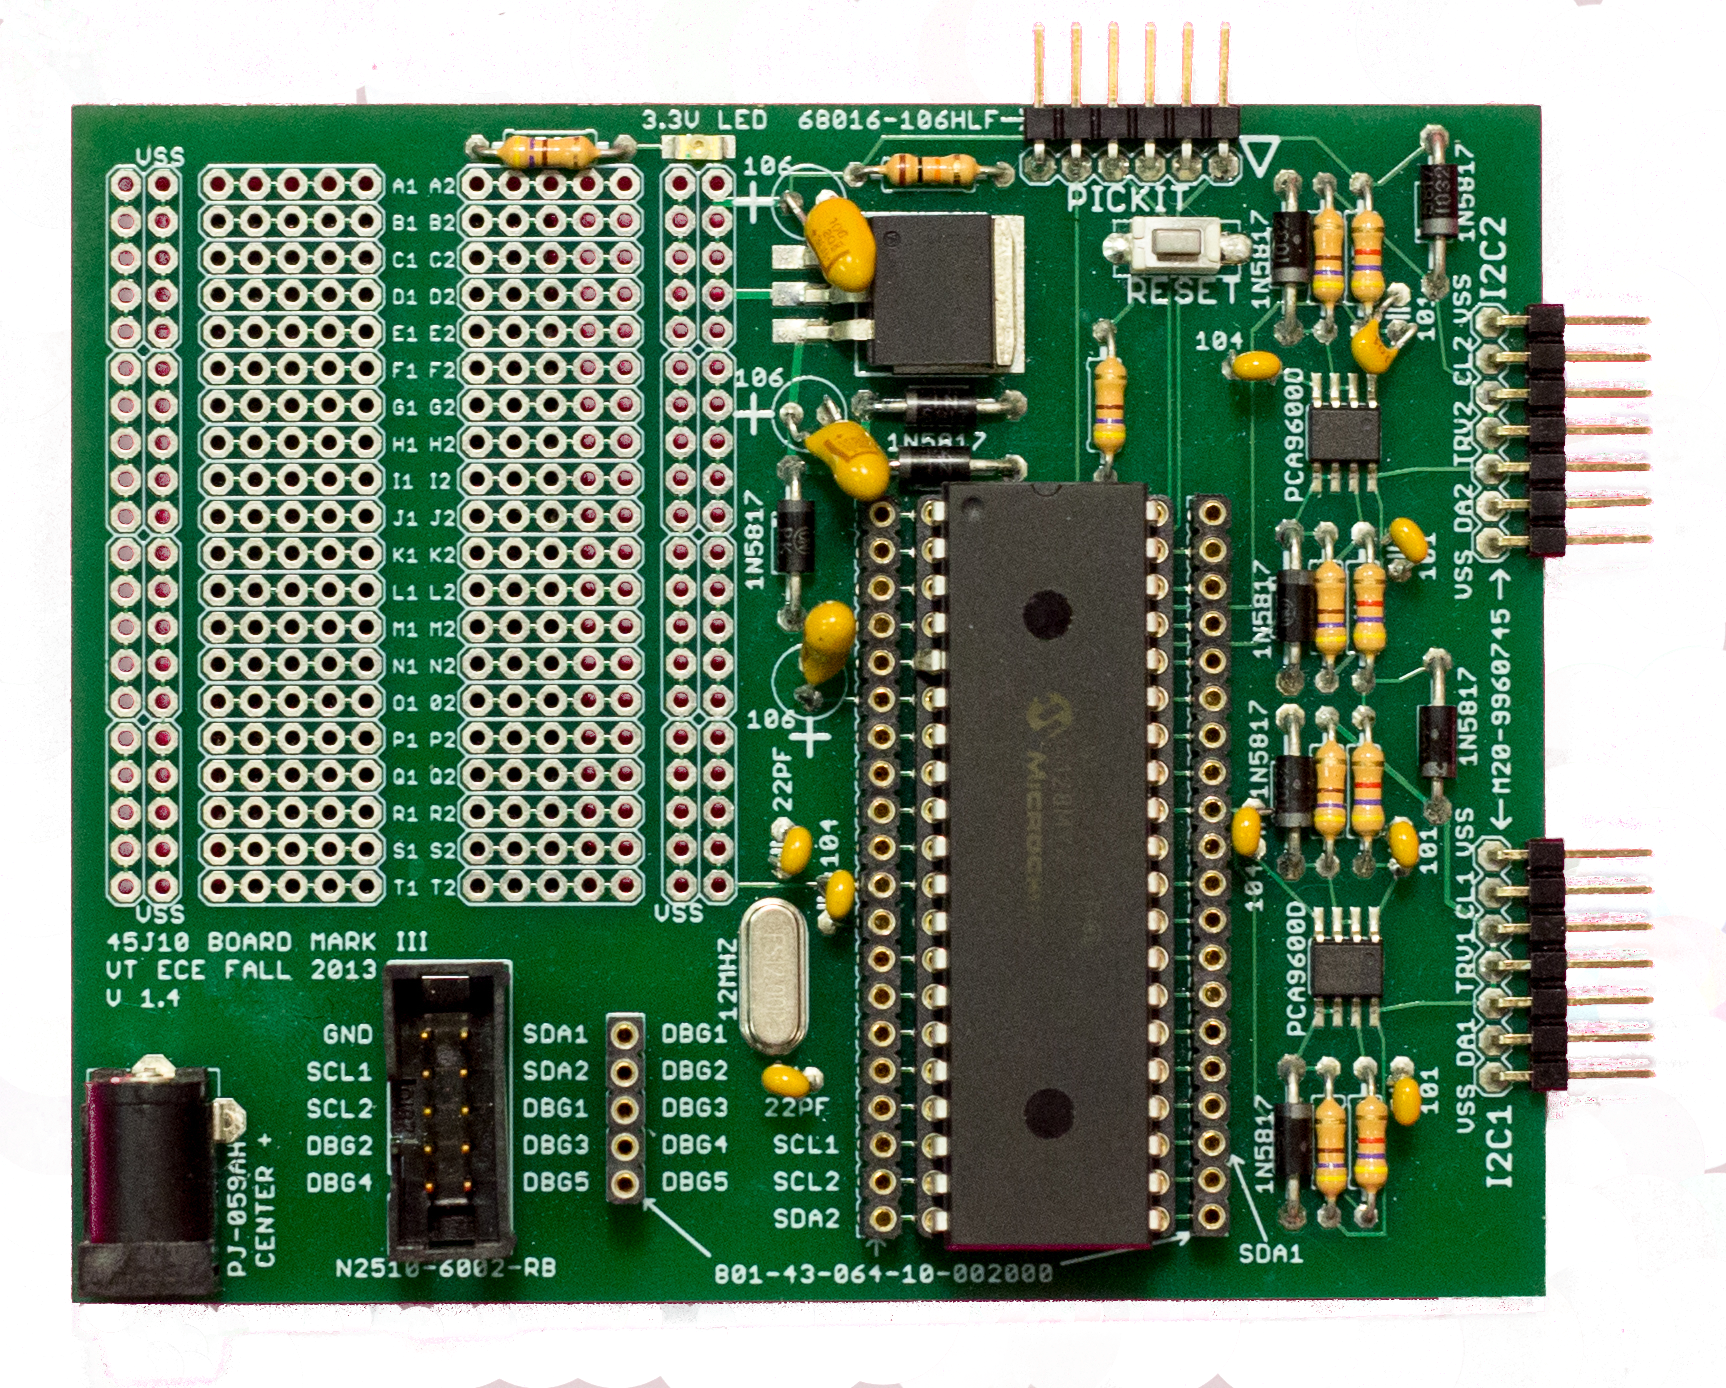
\includegraphics[scale=0.35]{Images/mark3.png}
	PIC18F45J10
\end{center}
\begin{center}
	\includegraphics[scale=0.35]{Images/motorcontroller.png}
	Sabertooth 2x12 Motor Controller
\end{center}
\begin{center}
	\includegraphics[scale=0.35]{Images/motor.png}
	Motor PIC
\end{center}
\begin{center}
	\includegraphics[scale=0.35]{Images/sensor.png}
	Sensor PIC
\end{center}
\begin{center}
	\includegraphics[scale=0.35]{Images/rover.png}
	Top view of rover
\end{center}

\subsection{Conclusion}

\end{document}
